%!TEX root = ../PhDThesis.tex



% *********************************************************************************************************************
\chapter{Additional information about the third study}\label{app:studyinfo-home}
% *********************************************************************************************************************



This appendix includes additional material to the third study of \acf{VUI} use in a home (see \autoref{ch:empirical home}):

\begin{itemize}
    \item \appref{app:studyinfo-home infoconsent} provides the information sheet and consent form given to participants prior to the study, and
    \item \appref{app:studyinfo-home helpguide} provides the Amazon Echo Help Guide produced for the study, and left with participant households.
\end{itemize}



% *********************************************************************************************************************




\includepdf[
    pages={1},
    scale=.6,
    frame=false,
    clip,
    trim=1.5cm 1.5cm 1.5cm 1.5cm,
    pagecommand={\section{Information sheet and consent form}\label{app:studyinfo-home infoconsent}}]
    {Graphics/D-StudyInfo-Home/InfoConsent.pdf}

\includepdf[
    pages={2},
    scale=.6,
    frame=false,
    clip,
    trim=1.5cm 1.5cm 1.5cm 1.5cm,
    pagecommand={\nopagebreak}]
    {Graphics/D-StudyInfo-Home/InfoConsent.pdf}



% *********************************************************************************************************************



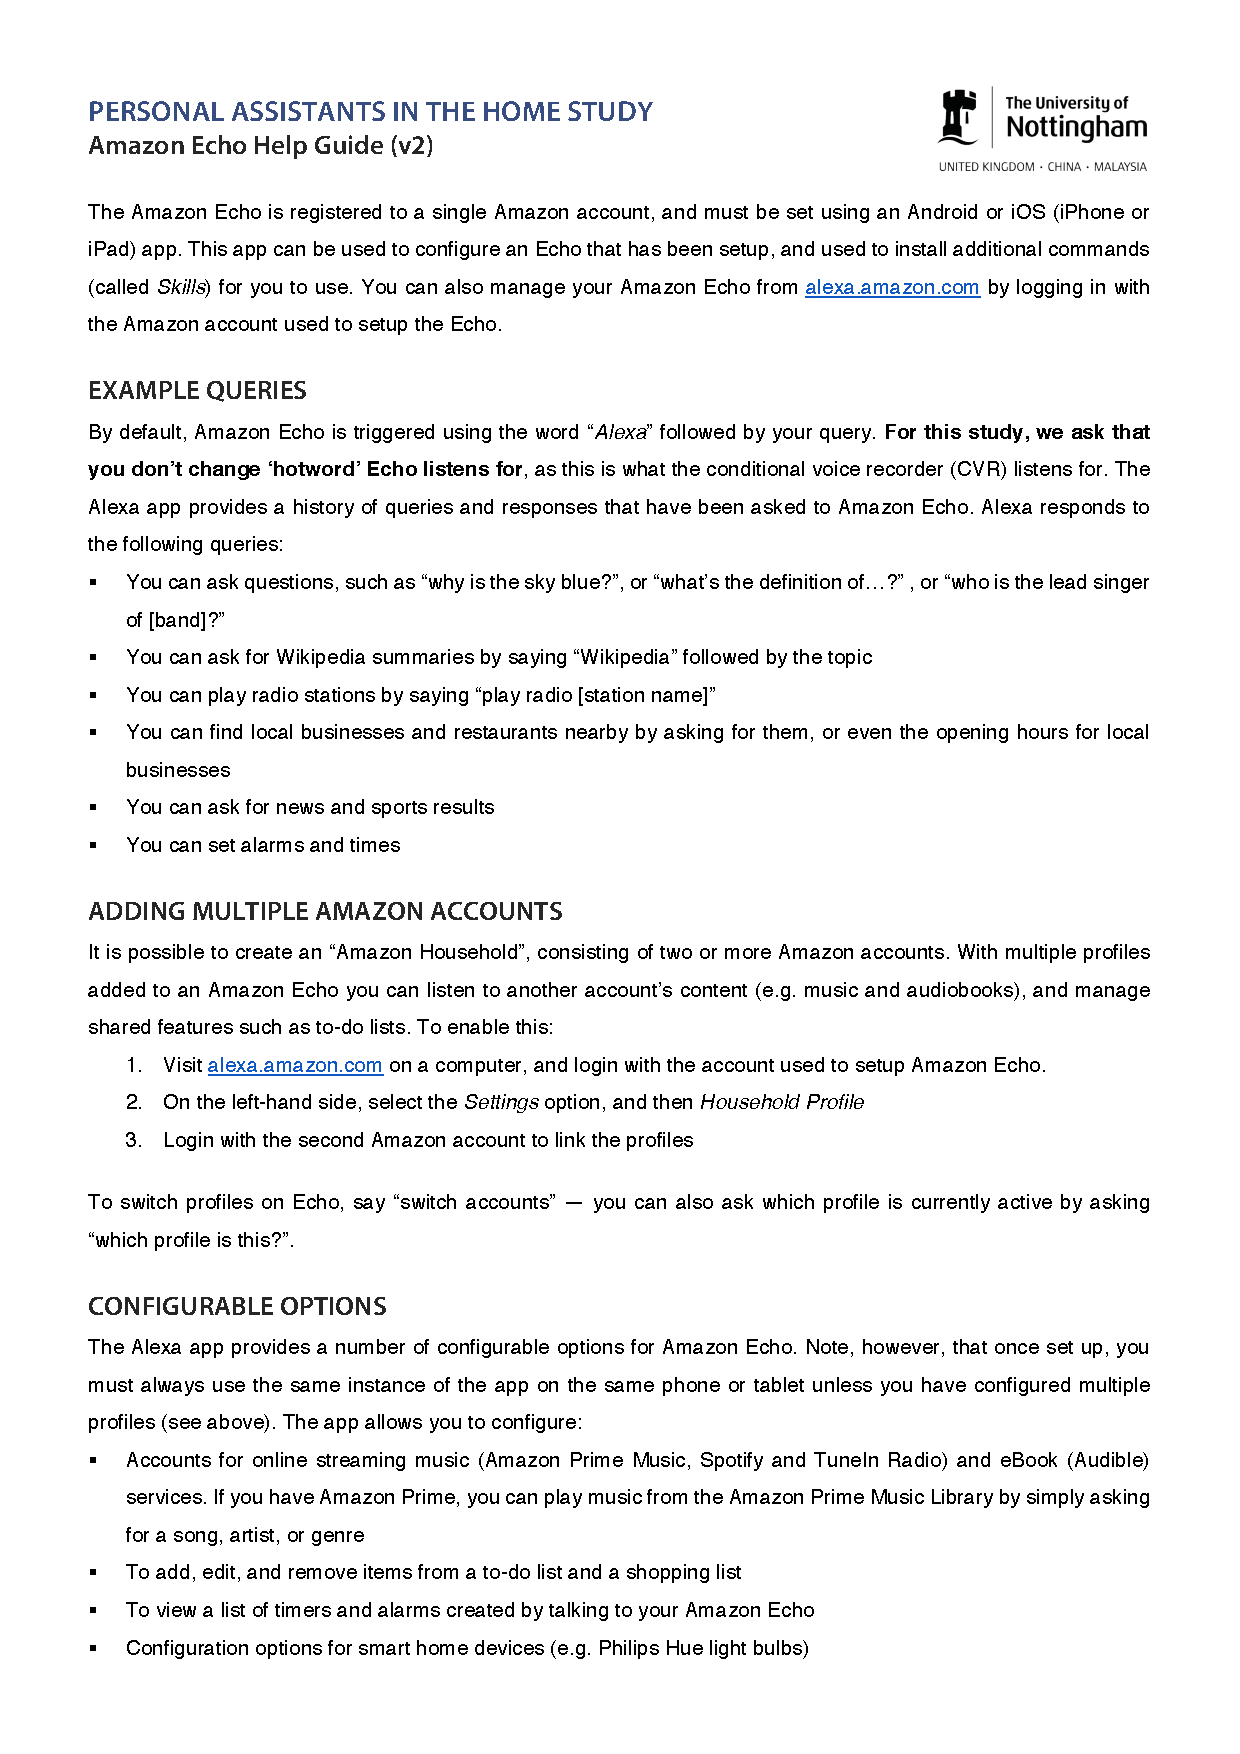
\includepdf[
    pages={1},
    scale=.6,
    frame=false,
    clip,
    trim=1.5cm 1.5cm 1.5cm 1.5cm,
    pagecommand={\section{Amazon Echo help guide}\label{app:studyinfo-home helpguide}}]
    {Graphics/D-StudyInfo-Home/AmazonEchoHelpGuide.pdf}
\includepdf[
    pages={2},
    scale=.6,
    frame=false,
    clip,
    trim=1.5cm 1.5cm 1.5cm 1.5cm,
    pagecommand={\nopagebreak}]
    {Graphics/D-StudyInfo-Home/AmazonEchoHelpGuide.pdf}



% *********************************************************************************************************************


% \section{Exit Interview Questions}\label{app:studyinfo-home interview}
% Exit Interviews with participants were performed roughly one-week after data capture ended, and was with the primary occupants of the household.
% The interview was split into two sections: (1) general questions, (2) reflection on selected queries.



% *********************************************************************************************************************


% \subsection*{General Questions}
% The following questions were asked to all participants in the study through a semistructured interview unless answered in a previous question.

% \begin{itemize}
%   \item What were your general impressions of using Echo in your home?
%   \begin{itemize}
%   \item Did you use it much?
%   \item Did you feel it affected your privacy?
%   \end{itemize}

%   \item What sort of queries did you ask of Echo?
%   \begin{itemize}
%   \item Who used it?
%   \item What did you use it for?
%   \item What did you ask?
%   \end{itemize}

%   \item How did you discover what questions you could ask?
%   \item Did you find the Echo was particularly good at recognising what you asked it to do?
%   \item When did you think the Echo was struggling?
%   \item Did Echo respond accordingly to what you asked it to do?
%   \item If you could ask Echo to do anything, what would it be? Were they times you wanted it to do something you couldn’t?
%   \item Were there times when Echo did stuff unexpectedly?

%   \item When Echo failed to respond to a query, how did find Echo’s response?
%   \item Did you understand what went wrong? Did you try and resolve the problem?

%   \item Did guests, friends, or other family members talk to Echo? Were you happy for this to happen?
%   \item Did they understand how to talk to it or did you provide explanations?
%   \item What sort of queries did they ask?
%   \item What was your experience of multiple people using Echo? Can you give an example?
% \end{itemize}

% \subsection*{Reflection on Selected Queries}
% A number of episodes were selected which involved potentially interesting findings, and each one was played to the participants as a probe to gauge further reflection.

% \begin{itemize}
%   \item Could you, in your own words, describe the interaction? What did you think about what happened?
%   \item What would you say motivated the query?
%   \item What did you think about Echo’s response?
%   \item How do you think Echo should have responded?
% \end{itemize}

% If query was worded by other than the interviewee(s), the following questions were asked:

% \begin{itemize}
%   \item How did you feel about the person asking the query?
%   \item What was your perception of Echo’s response?
% \end{itemize}

% If follow-up query was performed by other than the initial query performer, the following questions were asked:

% \begin{itemize}
%   \item What did you think about the follow-up query?
%   \item Why was the query repeated/refined? (choose appropriate)
%   \item How did you negotiate another person asking the query? (i.e. did it just happen or was it to explain or show people how it worked?)
% \end{itemize}



% *********************************************************************************************************************
